\chapter{Modellentwurf}\label{sec:modellentwurf}
Nachdem nun alle notwendigen Grundlagen erläutert wurden, wird in diesem Kapitel der Grid Fin samt Aktuatorik entworfen. Hierzu werden zunächst die Anforderungen an das System aufgestellt, um dann auf dieser Basis eine geeignete Wahl der Designvarianten treffen zu können. Zur Übersicht über die verschiedenen technischen Umsetzungsvarianten wird ein morphologischer Kasten zur Hilfe gezogen. Schlussendlich wird in Abschnitt \ref{sec:modelldesign} ein erstes Modell zusammengestellt und anschließend in CAD modelliert.
\section{Systemanforderungen}
Zunächst werden also die Anforderungen an das System definiert. Hierbei wird sich hauptsächlich auf eine in MatLab mit Simulink durchgeführte Simulation und Angaben von GAIA Aerospace bezogen.
\subsection{Leistungsanforderungen}
Aerodynamsiche Leistung
Motorleistung
\subsection{Anforderungen an die Kosten}
\subsection{Thermische Anforderungen}
\subsection{...}

\section{Morphologischer Kasten}
Um eine Übersicht über die verschiedenen Designmöglichkeiten zu haben wird an dieser Stelle ein morphologischer Kasten, wie in er in Abbildung \ref{abb_MorphKast} zu sehen ist, eingeführt. Für acht Designentscheidungen sind dort unterschiedliche Teillösungen aufgelistet. Ganz links sind drei mögliche Zellformen gegeben. Es besteht die Wahl zwischen quadratischen, drei- und sechseckigen Geometrien. Hierbei sei aber wieder zu berücksichtigen, dass es auch zu einen Mischung mehrerer Formen kommen kann und besonders am Rand durch den Rahmen die Zellen ungleichmäßig verkleinert werden könnten.

Für die Form des gesamten Gitters stehen nur zwei unterschiedliche Möglichkeiten zur Auswahl: Rechteck oder Diamant. Da jedoch die Maße noch nicht festgelegt sind kann die ersten der beiden Formen auch noch zum Quadrat werden. Des Weiteren kann es sein, dass die Geometrie an der einen Seite für die Anbringung noch angepasst wird.

Die größte Auswahl bietet sich bei den Wandquerschnittsformen. Rechteckig, abgerundet, beidseitig und einseitig spitzt, trapezförmig und dreieckig sind die sechs Optionen, die es hier gibt. Der Wandquerschnitt muss nicht überall die gleiche Form besitzen. So kann es kommen, dass das Gitter eine unterschiedliche erhält als der Rahmen. Die unteren beiden Formen sind zum Beispiel asymmetrisch, sodass sie nur für die Umrandung der Grid Fins in Frage kommen.

Als viertes wird die Fragestellung einer Krümmung gezeigt. Neben einem flachen Design kann der Grid Fin entweder zur Strömung hin konvex oder konkav gekrümmt sein. Dies ist abhängig davon in welche Richtung die Finne eingeklappt werden kann.

Im Grundlagenkapitel wurden drei verschiedene Arten der Pfeilung eines Grid Fins gezeigt. Da sie sich grundsätzlich unterschiedlich implementieren lassen, können sie theoretisch sogar in Kombination gewählt werden. Der Pfeilungswinkel ist ist für die Varianten noch frei wählbar und auch negative Winkel, also Vorwärtspfeilung, ist denkbar. Für die lokale Pfeilung der Zellen rückt der Unterschied zwischen Vorwärts- und Rückwärtspfeilung durch die Unterscheidung vom Berg- und Tal-Typus noch mehr in den Vordergrund. Wichtig ist noch anzumerken, dass die konfigurelle Pfeilung keinen direkten Einfluss auf das Design der Grid Fins an sich hat, sondern sich durch den Bewegungsspielraum der Aktuatorik umsetzten lässt.

Eine wichtige Designentscheidung ist der Aktuator, da er bestimmt was als Energiequelle genutzt wird und hat somit einen großen Einfluss auf Gewicht und Kosten. Eine Möglichkeit ist die elektrische Energie zu nutzen und diese mit einem Elektromotor direkt die mechanische Arbeit verrichten zu lassen. Alternativ kann auch ein hydraulisches oder gar pneumatisches System verwendet werden. Da Grid Fins zwei Freiheitsgrade haben, können diese über unterschiedliche Aktuatoren, die auch unterschiedlicher Art sein können, bewegt werden. Also muss in diesem Punkt für beide Rotationen einzeln entschieden werden.

Über ein Getriebe wird die Leistung des Aktuators auf die Grid Fins übertragen, um mehr Spielraum für Kraft, Moment, Drehzahl und Orientierung des Aktuators zu gewährleisten. Eine Möglichkeit bietet das klassische Zahnradgetriebe. Viele Paarungen, wie zum Beispiel Kegelräder, Schneckenräder und viele weitere, sind denkbar. Kräfte und die zugehörige Bewegungsgeschwindigkeit lassen sich durch hydrostatische Getriebe beeinflussen. Momente und Drehzahlen können durch hydrodynamische Getriebe verändert werden. Generell sind durch Kombinationen beliebig komplexe Systeme möglich

Als letztes beschäftigt sich der Morphologische Kasten in Abbildung \ref{abb_MorphKast} mit der Lagerung. Hierbei wird generell zwischen den Wälz- und Gleitlagern unterschieden. Beide bieten jedoch noch mehr Entscheidungsfreiheiten. So gibt es einige unterschiedliche Wälzkörper, wie Kugeln, Zylinder, Kegel, etc.. Auch Gleitlagern können weiter zu statischen und dynamischen unterteilt werden, je nach Art der Schmierfilmdruckerzeugung.
\\~\\
Es gibt jedoch noch weitere Designentscheidungen, die sich nicht in einem morphologischen Kasten pragmatisch darstellen lassen. So müssen zum einen noch die Dimensionen des Moduls und Lage der Aktuatoren in der Rakete definiert werden. Zum anderen stellt sich die Frage welche Zellgröße $g$ und Wandstärke $d$ an welcher Stelle gewählt wird. Es besteht auch noch die Möglichkeit die Grid Fins mit zusätzlichen Features auszustatten. Eine Option wären hier zusätzliche Stützstreben oder sogar durch die additive Fertigung ermöglichte, in das Material integrierte Strukturen, wie zum Beispiel Kühlkanäle oder Drucksensoren.
\begin{figure}[h]
	\centering
	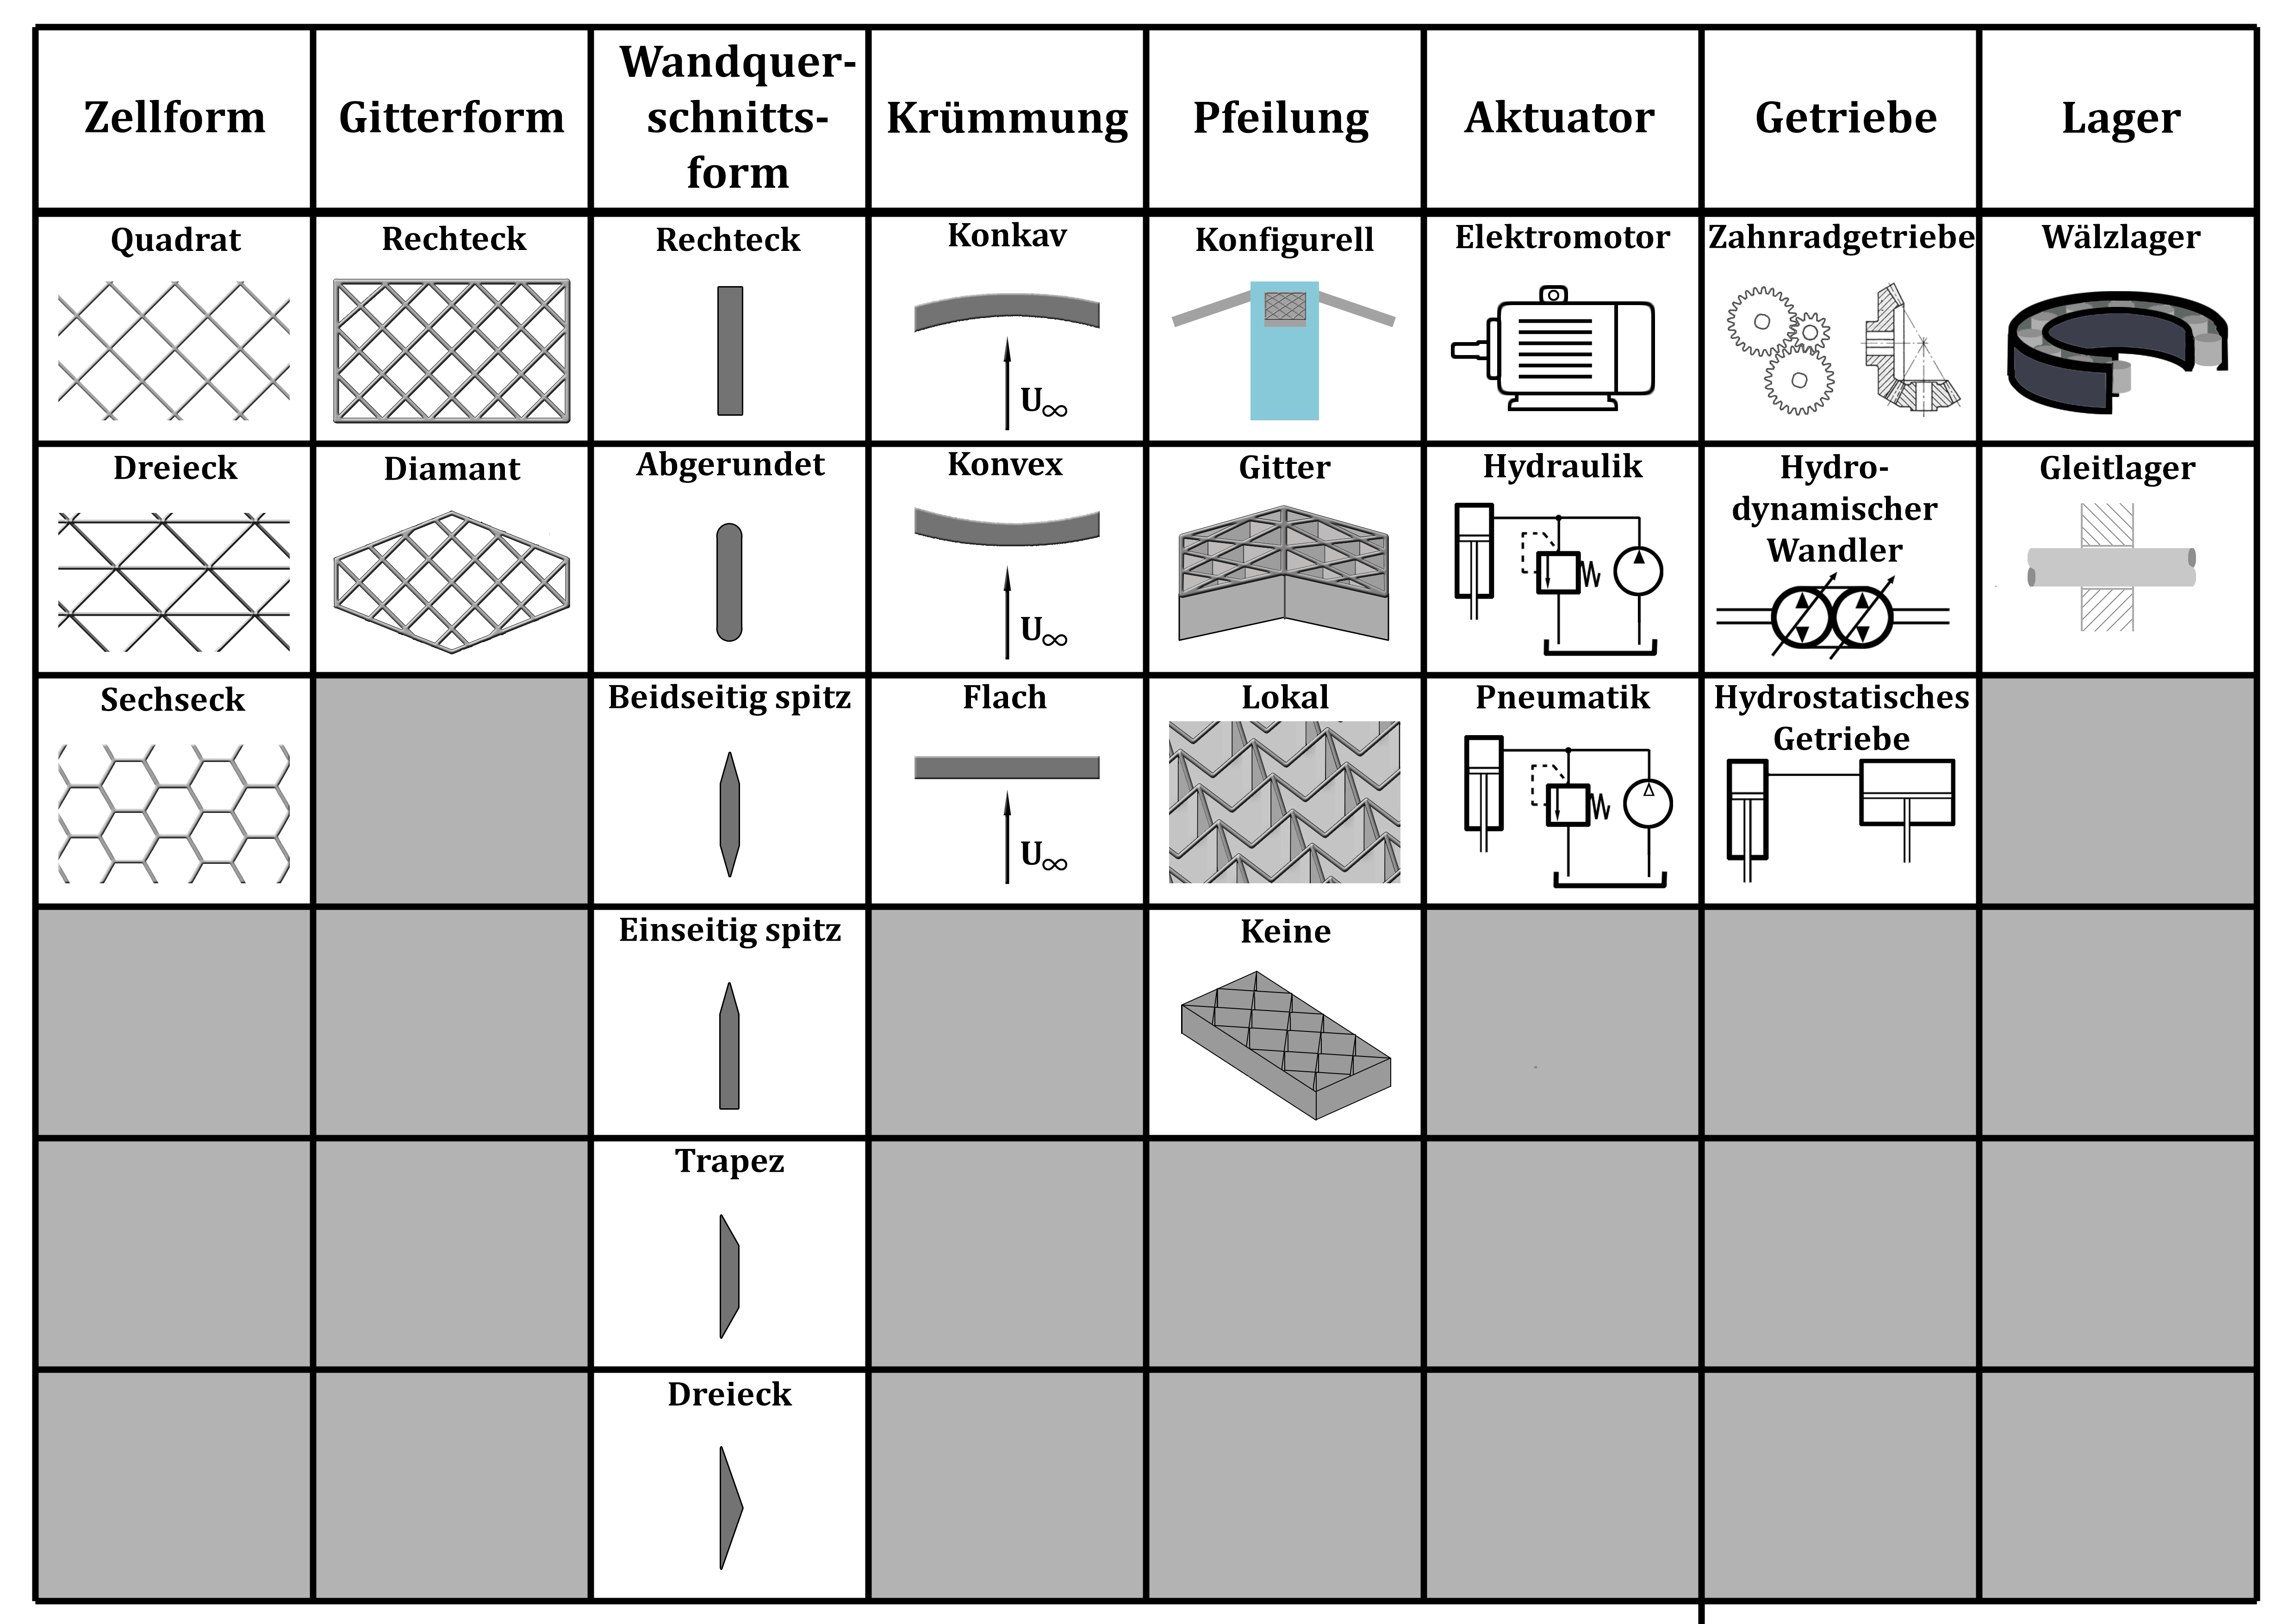
\includegraphics[angle=90, width=0.9\textwidth]{Morphologischer Kasten.png}
	\caption{Morphologischer Kasten für Grid Fin Aktuatorik}
	\label{abb_MorphKast}
\end{figure}
\newpage
\section{Komponentenrecherche und -auswahl}
\subsection{Gitterdesign}
\subsection{Aktuator}
\subsection{Getriebe}
\subsection{Peripherie}
z.B. Energieversorgung

\section{Festlegung des Modelldesigns}\label{sec:modelldesign}
Gesamtgröße
gap-to-chord
Pfeilungswinkel
Kanäle
Die additive Fertigung des Grid Fins ermöglicht neue Optionen, die für klassische Herstellungsverfahren nicht wirtschaftlich umsetzbar sind. So können zum Beispiel Kanäle in das Material integriert werden, welche genutzt werden können, um den Werkstoff zu kühlen oder gar das Air Flush System mit weiteren Drucksensoren ergänzen.

\section{Modellierung des Modells}